%%%%%%%%%%%%%%%%%%%%%%%%%%%%%%%%%%%%%%%%%
% Beamer Presentation
% LaTeX Template
% Version 1.0 (10/11/12)
%
% This template has been downloaded from:
% http://www.LaTeXTemplates.com
%
% License:
% CC BY-NC-SA 3.0 (http://creativecommons.org/licenses/by-nc-sa/3.0/)
%
%%%%%%%%%%%%%%%%%%%%%%%%%%%%%%%%%%%%%%%%%

%----------------------------------------------------------------------------------------
%	PACKAGES AND THEMES
%----------------------------------------------------------------------------------------

\documentclass{beamer}

\mode<presentation> {

% The Beamer class comes with a number of default slide themes
% which change the colors and layouts of slides. Below this is a list
% of all the themes, uncomment each in turn to see what they look like.

%\usetheme{default}
%\usetheme{AnnArbor}
%\usetheme{Antibes}
%\usetheme{Bergen}
\usetheme{Berkeley}
%\usetheme{Berlin}
%\usetheme{Boadilla}
%\usetheme{CambridgeUS}
%\usetheme{Copenhagen}
%\usetheme{Darmstadt}
%\usetheme{Dresden}
%\usetheme{Frankfurt}
%\usetheme{Goettingen}
%\usetheme{Hannover}
%\usetheme{Ilmenau}
%\usetheme{JuanLesPins}
%\usetheme{Luebeck}
%\usetheme{Madrid}
%\usetheme{Malmoe}
%\usetheme{Marburg}
%\usetheme{Montpellier}
%\usetheme{PaloAlto}
%\usetheme{Pittsburgh}
%\usetheme{Rochester}
%\usetheme{Singapore}
%\usetheme{Szeged}
%\usetheme{Warsaw}

% As well as themes, the Beamer class has a number of color themes
% for any slide theme. Uncomment each of these in turn to see how it
% changes the colors of your current slide theme.

%\usecolortheme{albatross}
%\usecolortheme{beaver}
%\usecolortheme{beetle}
%\usecolortheme{crane}
%\usecolortheme{dolphin}
%\usecolortheme{dove}
%\usecolortheme{fly}
%\usecolortheme{lily}
%\usecolortheme{orchid}
%\usecolortheme{rose}
%\usecolortheme{seagull}
%\usecolortheme{seahorse}
%\usecolortheme{whale}
%\usecolortheme{wolverine}

%\setbeamertemplate{footline} % To remove the footer line in all slides uncomment this line
%\setbeamertemplate{footline}[page number] % To replace the footer line in all slides with a simple slide count uncomment this line

%\setbeamertemplate{navigation symbols}{} % To remove the navigation symbols from the bottom of all slides uncomment this line
}

\usepackage{graphicx} % Allows including images
\usepackage{hyperref}
\usepackage{mwe}
\usepackage{natbib}
\usepackage{tabu}
\usepackage{booktabs} % Allows the use of \toprule, \midrule and \bottomrule in tables

%----------------------------------------------------------------------------------------
%	TITLE PAGE
%----------------------------------------------------------------------------------------

\title[Ensemble Visualization]{Ensemble Forecast Visualization and Verification in Python} % The short title appears at the bottom of every slide, the full title is only on the title page

\author{Tyler Wixtrom} % Your name
\institute[TTU/ATMO] % Your institution as it will appear on the bottom of every slide, may be shorthand to save space
{
Atmospheric Sciences Group, Texas Tech University \\ % Your institution for the title page
\medskip
\textit{tyler.wixtrom@ttu.edu} % Your email address
}
\date{\today} % Date, can be changed to a custom date

\begin{document}

\begin{frame}
\titlepage % Print the title page as the first slide
\end{frame}

\begin{frame}
\frametitle{Overview} % Table of contents slide, comment this block out to remove it
\tableofcontents % Throughout your presentation, if you choose to use \section{} and \subsection{} commands, these will automatically be printed on this slide as an overview of your presentation
\end{frame}

%----------------------------------------------------------------------------------------
%	PRESENTATION SLIDES
%----------------------------------------------------------------------------------------
\begin{frame}
  \frametitle{Examples and Data Repository}
  \url{https://github.com/tjwixtrom/workshop2018}
\end{frame}

%------------------------------------------------
\section{Plots} % Sections can be created in order to organize your presentation into discrete blocks, all sections and subsections are automatically printed in the table of contents as an overview of the talk
%------------------------------------------------

\subsection{Spaghetti Plots and Postage Stamps} % A subsection can be created just before a set of slides with a common theme to further break down your presentation into chunks

\begin{frame}
\frametitle{Spaghetti Plots and Postage Stamps}
Spaghetti plots and postage stamp plots are both concise, simple methods of viewing all members in a ensemble on the same plot. Spaghetti plots are generally used for contoured fields (e.g. 500 hPa geopotential height) while postage stamps are more commonly reserved for shaded fields (e.g. simulated reflectivity).

%\begin{figure}
%    \centering
%    \begin{minipage}{0.45\textwidth}
%        \centering
%        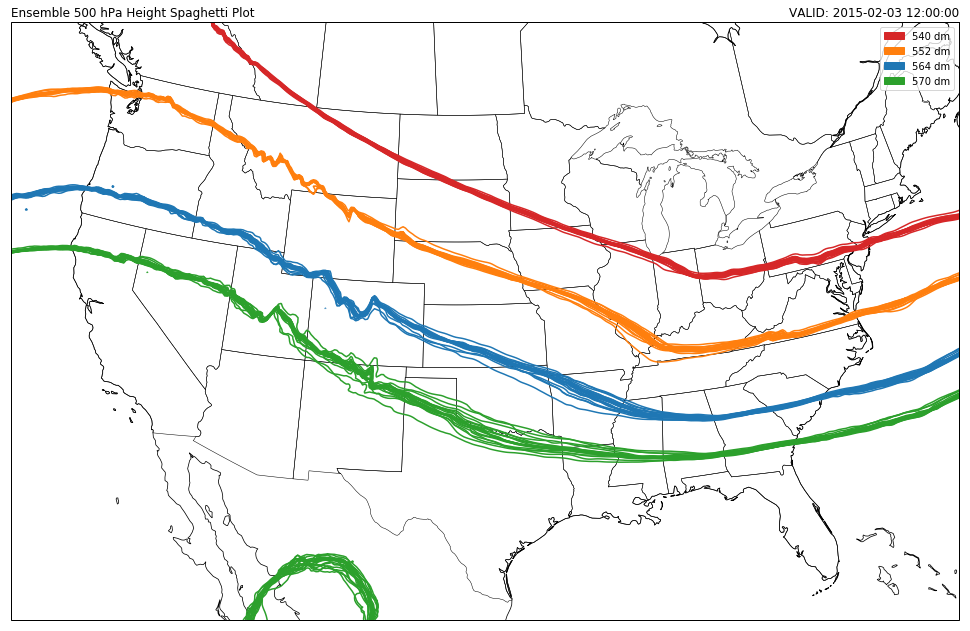
\includegraphics[width=0.8\textwidth]{spaghetti} % first figure itself
%    \end{minipage}\hfill
%    \begin{minipage}{0.45\textwidth}
%        \centering
%        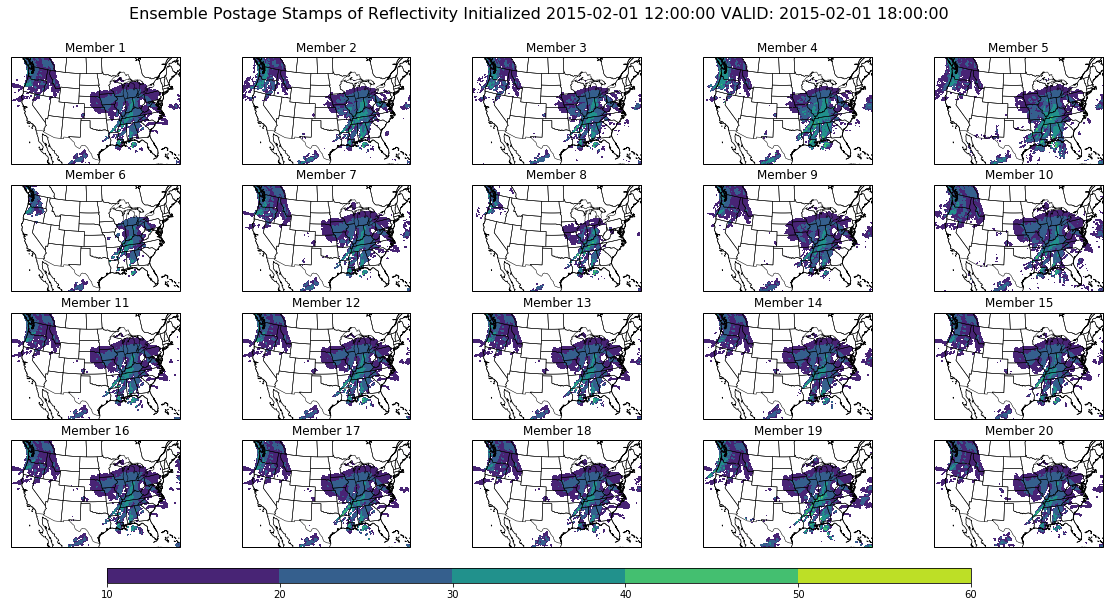
\includegraphics[width=0.9\textwidth]{postage_stamp} % second figure itself
%    \end{minipage}
%\end{figure}

\end{frame}

\begin{frame}
  \frametitle{Spaghetti Plots and Postage Stamps}
  \begin{figure}
    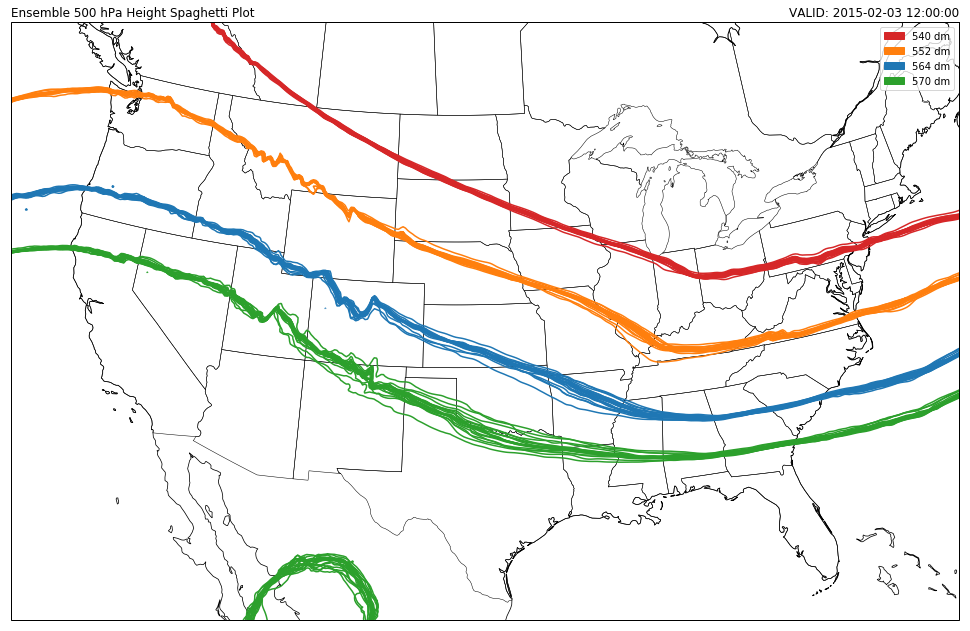
\includegraphics[width=0.8\textwidth]{spaghetti}
  \end{figure}
\end{frame}

\begin{frame}
  \frametitle{Spaghetti Plots and Postage Stamps}
  \begin{figure}
    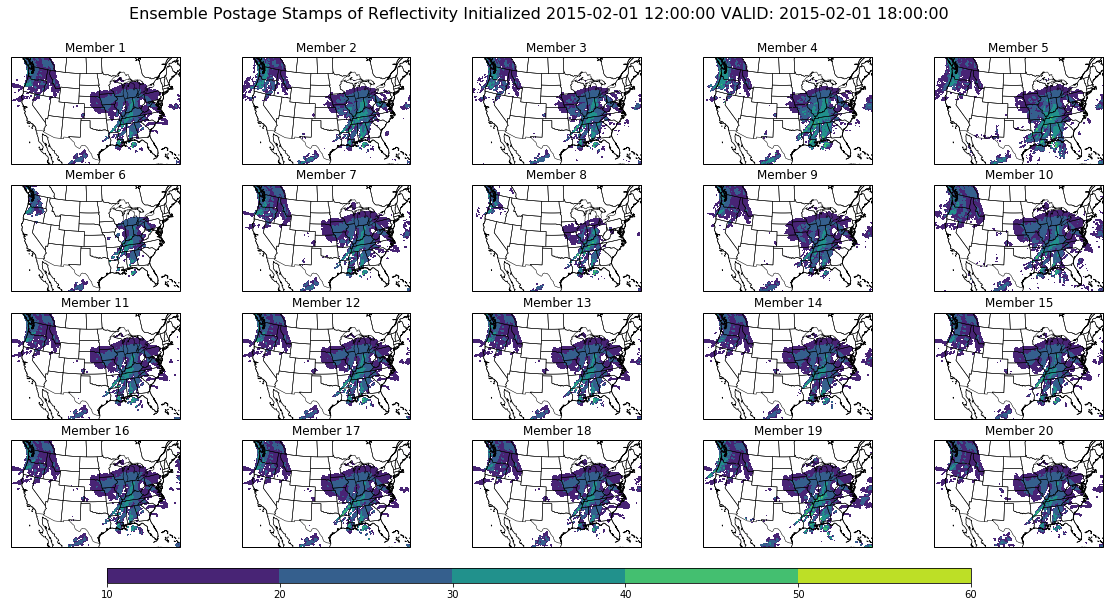
\includegraphics[width=0.8\textwidth]{postage_stamp}
  \end{figure}
\end{frame}

%------------------------------------------------
\begin{frame}
\frametitle{Spaghetti Plots and Postage Stamps}
Advantages
\begin{itemize}
\item Displays information from each individual member
\item Full location and magnitude of each field is plotted
\item Simple to interpret 
\end{itemize}

Disadvantages
\begin{itemize}
  \item Can be very busy
  \item Becomes increasingly hard to interpret as spread increases
  \item Easy to miss small differences among members (esp. postage stamps)
\end{itemize}
\end{frame}

%------------------------------------------------
\subsection{Paintball Plots}
\begin{frame}
\frametitle{Paintball Plots}
Paintball plots are plots where individual points greater than a specified threshold (e.g. simulated reflectivity $\geq$ 40 dBZ) are plotted, color-coded by ensemble member.

\begin{figure}
    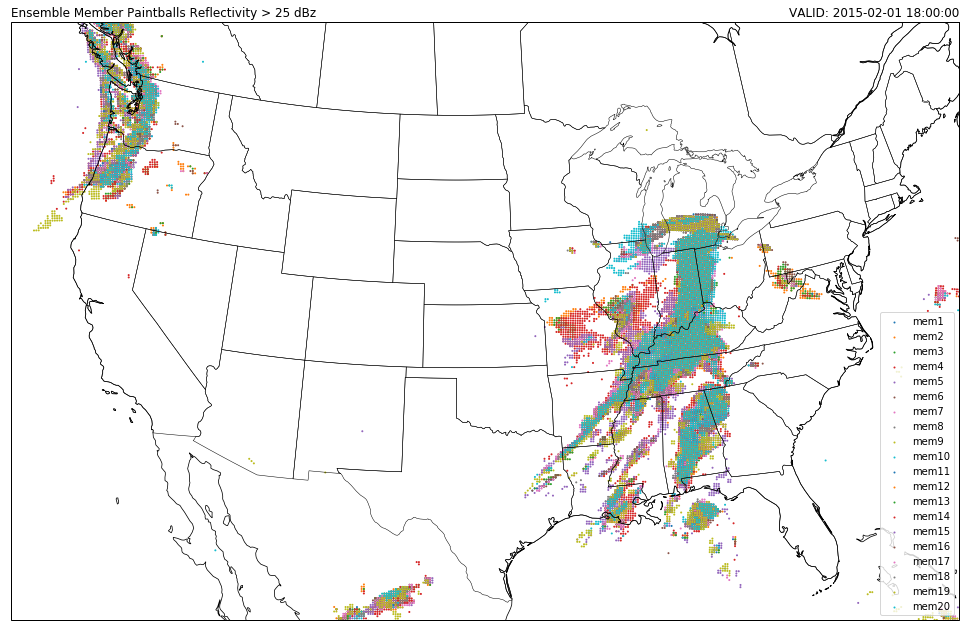
\includegraphics[width=0.8\textwidth]{paintballs}
\end{figure}
\end{frame}

\begin{frame}
  \frametitle{Paintball Plots}
  Advantages
  \begin{itemize}
    \item Easy to quickly see spatial variations among individual member solutions
    \item Plot remains relatively uncluttered, even for ensembles with many members
  \end{itemize}
  Disadvantages
  \begin{itemize}
    \item Very little information regarding variations in intensity
    \item Thresholds are arbitrary and may not be best for all cases
  \end{itemize}
\end{frame}

\subsection{Probability Plots}

\begin{frame}
  \frametitle{Probability Plots}
  If an ensemble contains a sufficient number of members and sufficient spread, probabilities of event occurence can be calculated based on the individual members. This is done at a single point with the following method \citep{Schwartz2017}:
\end{frame}


\begin{frame}
  \frametitle{Ensemble Probability}
\begin{itemize}
 \item Define threshold for field
 \item Define the binary probability (BP) at each point
 \begin{equation}
    BP(q)_{ij} = \left\{
        \begin{array}{ll}
            1 & \quad f_{ij} \geq q \\
            0 & \quad f_{ij} < q
        \end{array}
    \right.
   \end{equation} 

\item Take average of member binary probabilities to define ensemble probability (EP) for each point
\begin{equation}
     EP(q)_{i} = \frac{1}{N}\sum^{N}_{j=1}BP_{ij}
   \end{equation}
\end{itemize}
\end{frame}  

\begin{frame}
  \frametitle{Ensemble Probability}
  \begin{figure}
    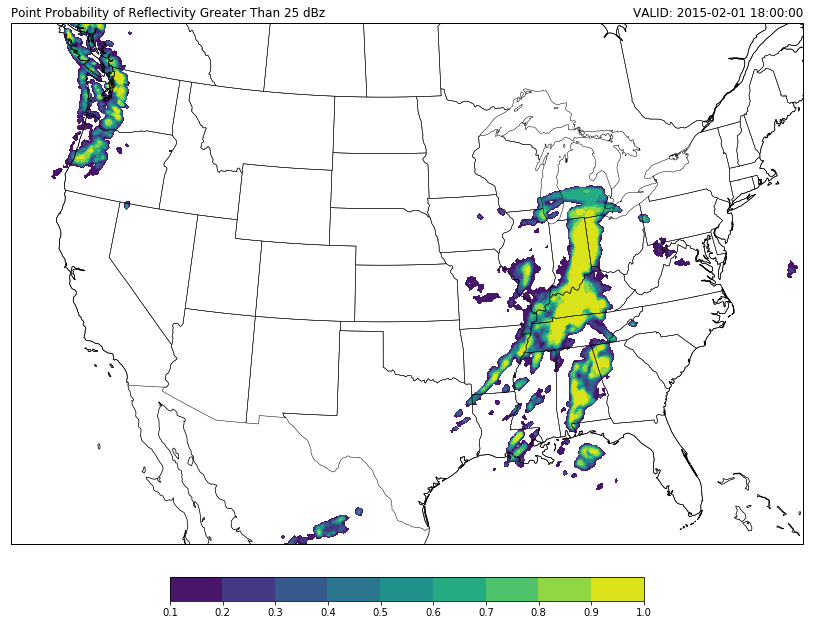
\includegraphics[width=0.8\textwidth]{probs}
\end{figure}
\end{frame}

\begin{frame}
  \frametitle{Neighborhood Ensemble Probability}
  Since the ensemble probability is defined for only a single point and does not account for spatial differences in member solutions, the Neighborhood Ensemble Probability (NEP) can be defined as the probability of even occurence within a specified radius of any point \citep{Schwartz2017}. 
\end{frame}

\begin{frame}
  \frametitle{Neighborhood Ensemble Probability}
  To calculate the NMEP for a given field and threshold $q$:
  \begin{itemize}
    \item Begin by calculating the EP at each point
    \item Find all points within specified radius and calculate mean of EP
    \begin{equation}
      NEP(q)_{i} = \frac{1}{N_b}\sum^{N_b}_{j=1}EP_{ij}
    \end{equation}
  \end{itemize}
\end{frame}

\begin{frame}
  \frametitle{Neighborhood Ensemble Probability}
  \begin{figure}
    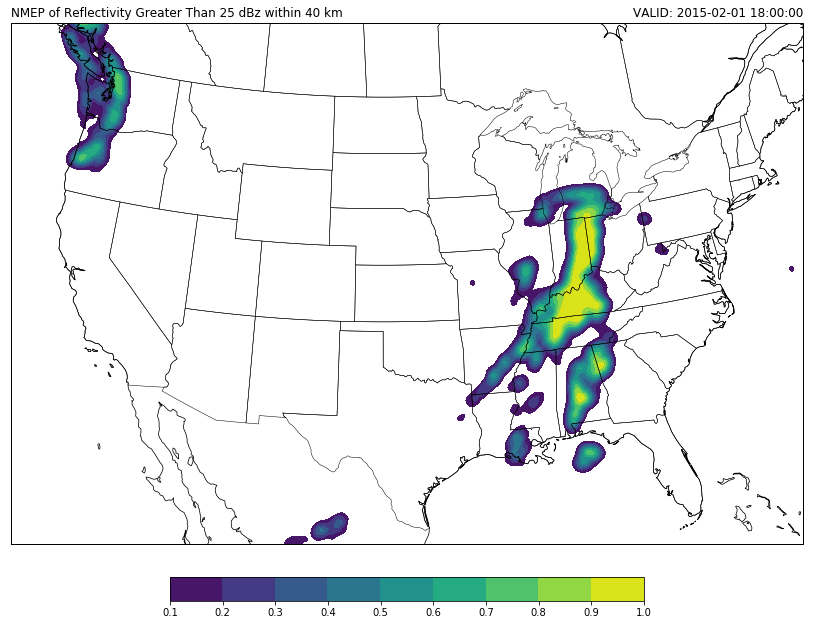
\includegraphics[width=0.8\textwidth]{neighbor_probs}
  \end{figure}
\end{frame}

\begin{frame}
  \frametitle{Probability Plots}
  Advantages
  \begin{itemize}
    \item Probabilistic forecasts of specific events
    \item Quickly shows ensemble confidence
    \item Relatively simple to interpret
  \end{itemize}
  Disadvantages
  \begin{itemize}
    \item Probabilities are often too high due to low model spread
    \item Assumes that all member solutions are equally likely
    \item Limited information regarding member differences in intensity and location
  \end{itemize}
\end{frame}



\section{Verification}
\begin{frame}
  \frametitle{Verification}
  There are many verification metrics available which can be placed into three categories:
  \begin{itemize}
    \item Grid-point \citep{Wolff2014}
    \item Object-based \citep{Davis2006}
    \item Neighborhood approaches \citep{Schwartz2017}
  \end{itemize}
  One very simple approach that is often used in the Root Mean Square Error (RMSE).
\end{frame}

\subsection{RMSE}
\begin{frame}
  \frametitle{Root Mean Square Error}
  The Root Mean Square Error is defined as:
  \begin{equation}
    RMSE = \sqrt{\frac{1}{N}\sum_{i=1}^{N}(F_i - O_i)^2}
  \end{equation}
  \begin{itemize}
    \item Measure of mean magnitude of forecast error
    \item Same units as forecast value
    \item Simple to compute and interpret
    \item Useful for comparing two models, multiple members, etc.
    \item \cite{Holmes2000}
  \end{itemize}
\end{frame}

\section{Summary}
\begin{frame}
  \frametitle{Summary}
  \begin{center}

{\renewcommand{\arraystretch}{3}
   \begin{tabu} to 0.99\textwidth { | X[l, m] | X[l, m] | }
 \hline
 Plot Type & Best For \\ 
 \hline
 Spaghetti Plots and Postage Stamps & Individual members, spread, range of solutions \\ 
 \hline
 Paintballs & Differences in member spatial distribution \\
 \hline
 Probability & Likelihood of event occurence \\ 
 
 \hline
\end{tabu}}
\end{center}
\end{frame}

\section{Examples}
\begin{frame}
  \frametitle{Examples}
  \begin{enumerate}
    \item Open terminal
    \item Navigate to {\tt workshop2018} folder
    \item ``{\tt source activate workshop}'' for mac users, ``{\tt activate workshop}'' for windows users
    \item Type ``{\tt jupyter lab}''
  \end{enumerate}
\end{frame}
%------------------------------------------------
\begin{frame}
        \frametitle{References}
        \bibliographystyle{ametsoc}
        \small
        \bibliography{references}
\end{frame}

%------------------------------------------------
%
%\begin{frame}
%\Huge{\centerline{The End}}
%\end{frame}
%
%----------------------------------------------------------------------------------------

\end{document}